\chapter{مقدمه}

\section{تعمیر و نگهداری}

در دنیای نوین امروز، وابستگی به فناوری و صنایع مختلف برای ارائه خدمات و تولید محصولات مورد نیاز بشدت افزایش یافته‌است. در نتیجه این افزایش، تعداد کارخانه‌ها و تجهیزات برای رفع این نیازها نیز افزایش یافته‌است. همه تجهیزات و وسایل پس از استفاده زیاد دچار نقص و فراوانی می‌شوند. خرابی تجهیزات در کارخانه‌ها و حطوط تولید پدیده‌ای نامطلوب است. خرابی تجهیزات باعث ایست خط تولید و وارد کردن ضرر مالی به صاحبان کارخانه‌ها خواهد شد. به‌همین دلیل، تعمیر و نگهداری تجهیزات اهمیت بالایی دارد. 

سیاست‌های انجام تعمیرات و نگهداری به سه دسته اصلی تقسیم می‌شوند؛ که در \cref{MS} \cite{zhao2022review} آورده شده‌است:

\begin{figure}[!h]
\centering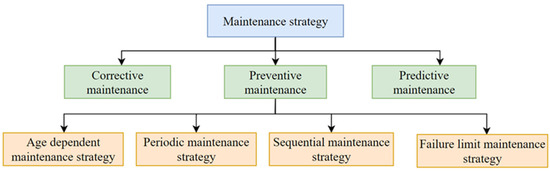
\includegraphics[scale=1]{maintenance_strategy.png}
\caption{سیاست‌های انجام تعمیرات و نگهداری \cite{zhao2022review}}\label{MS}
\end{figure}

این سیاست‌ها عبارتند از:
\begin{itemize}
\item نگهداری اصلاحی\LTRfootnote{Corrective Maintenance}: این نوع نگهداری با اتفاق افتادن خرابی رخ می‌دهد و تنها در صورت خرابی قطعه تعمیر انجام می‌شود. همانطور که مشخص است در این حالت روند کارکرد عادی متوقف می‌شود: به‌علاوه، در این حالت تعمیر می‌تواند با تاخیر انجام شود زیرا ممکن است در لحظه قطعات مورد نیاز برای تعمیر موجود نباشد. از این سیاست بیشتر به‌عنوان مکملی برای سیاست‌های بعدی استفاده می‌شود\cite{zhao2022review}.

\item نگهداری پیش‌گیرانه\LTRfootnote{Preventive Maintenance}: در این حالت، نگهداری و تعمیر بر اساس رابطه بین نرخ خرابی، توزیع زمان خرابی و سایر آستانه‌هایی که از تعداد زیادی از آمارهای خرابی بدست می‌آید زمان‌بندی می‌شود. در واقع در این نوع نگهداری هدف کاهش احتمال خرابی قطعات است. این نوع نگهداری با توجه به نوع اطلاعات به سیاست‌های وابسته عمر،\LTRfootnote{Age Dependent Strategies} سیاست‌های دوره‌ای\LTRfootnote{Periodic Strategies}، سیاست‌های ترتیبی\LTRfootnote{Sequential Strategies} و سیاست‌های محدودکننده خرابی\LTRfootnote{Failure Limited Strategies} تقسیم می‌شوند\cite{zhao2022review}.

\item نگهداری پیش‌بینانه\LTRfootnote{Predictive Maintenance}: این نوع نگهداری بر روند کاهش کارایی قطعات با استفاده از وضعیت آنها نظارت کرده، وضعیت آنها را در آینده پیش‌بینی می‌کند و مداوم برنامه تعمیر و نگهداری را بروزرسانی می‌کند، تا اینکه شرایط توقف بروزرسانی برآورده شود. با توجه به این ویژگی، این سیاست فقط برای تجهیزاتی که وضعیت آنها قابل نظارت است می‌تواند استفاده شود\cite{zhao2022review}.
\end{itemize} 

\section{راهکار پیشنهادی}

با توجه به اهمیت نگهداری و نقش نگهداری اصولی در کاهش هزینه، در این پروژه به ایجاد چارچوبی مناسب برای ارائه راهکاری بر مبنای سیاست نگهداری پیش‌بینانه می‌پردازیم. یکی از نیازهای این سیاست حجم زیادی از داده جمع‌آوری شده از وضعیت تجهیزات برای پیش‌بینی دقیق است. در این پروژه در بستر اینترنت اشیاء\LTRfootnote{Internet of Things} داده‌های لرزش با استفاده از سنسور \lr{MEMS}\LTRfootnote{Micro Electric Mechanical Sensor} جمع‌آوری شده و در زمان‌های مشخص با استفاده از پروتکل زیگبی\LTRfootnote{Zigbee Protocol} برای دروازه\LTRfootnote{Gateway} فرستاده می‌شود. پس از جمع‌آوری حجم مشخصی از داده‌هااطلاعات برای پردازش بیشتر به سرور فرستاده می‌شوند. در انتها نیز اطلاعات پردازش‌شده و تخمین عمر مفید باقیمانده\LTRfootnote{Remaining Useful Lifetime(RUL)} در یک صفحه وب نمایش داده می‌شود.

\section{کارهای مشابه}
در \cite{tinga2010application} مدلی برای خرابی قطعات مبتنی بر میزان استفاده از تجهیزات و بار داخلی آنها ارائه شده‌است اما مدل ارائه‌شده محدود به یک مدل تجهیزات است و برای استفاده در سایر مدل‌ها نظارت مجدد لازم است. در \cite{wu2007neural} رویکردی مبتنی بر شبکه عصبی جهت پیش‌بینی عمر مفید باقیمانده تجهیزات چرخشی ارائه شده‌است اما تنها مختص به این دسته از تجهیزات است. در \cite{kaiser2009predictive} رویکردی مبتنی بر شبکه عصبی جهت پیش‌بینی زمان نگهداری و تعمیرات تجهیزات بر اساس مدل خرابی و کارایی آنها ارائه می‌شود اما در یک محیط شبیه‌سازی‌شده و کنترل‌شده آزمایش شده‌است و در هنگام استفاده در محیط واقعی غیرعملی است.

بطور کلی در پژوهش‌های یادشده رویکرد‌های ارائه‌شده مختص نوع خاصی از تجهیزات است و در یک مجیط آزمایشگاهی و کنترل‌شده ارزیابی شده‌اند. در حالیکه در این پروژه با استفاده از داده‌های جمع‌آوری‌شده از قطعات مختلف سعی کرده‌ایم رویکردی کلی و مناسب محیط واقعی و صنعتی ارائه دهیم.
